%&template
\documentclass{article}
\usepackage{src/template}

\endofdump
\usepackage{minted}

\date{2025 -- 10 -- 26}
\useTemplate[NPA, Exercise=1]
\title{NPA -- Exercise 1}


\begin{document}
\maketitle

    \section{}

    \subsection{}

    % k parameter, even
    % Pod = Top switches + Bottom Switches
    % k/2 Backbone switches

    \begin{center}
        \def\podTop{4.5}
        \def\podBot{6}
        \def\podSep{0.15}
        
        \def\hostTop{8}
        \def\hostBot{11}
        \def\hostBetween{0.15}
        \def\hostSep{0.025}

        \begin{tikzpicture}

            \foreach \x in {1, ..., 3} {
                \foreach \y in {1, ..., 3} {
                    % Jedes j ist connected
                    \node[draw, minimum size=23pt] (backbone-\x-\y) at (\x*5+\y, 0) {$a_{\x,\y}$};
                }
            }

            \foreach \pod in {1, ..., 6} {
                \draw[color=Orchid, very thick] (\pod*3+0.45-\podSep, -\podTop+0.35 + \podSep) rectangle (\pod*3 + 3*0.8 + 0.35 + \podSep, -\podBot-0.35 - \podSep); % node[anchor=south, xshift=8pt] {$P_\pod$};
                % +0.45

                \foreach \x in {1, ..., 3} {
                    \node[circle, draw, inner sep=0pt, minimum size=20pt] (top-\pod-\x) at (\pod*3 + \x*0.8, -\podTop) {$t_{\pod,\x}$};

                    \node[circle, draw, inner sep=0pt, minimum size=20pt] (bottom-\pod-\x) at (\pod*3 + \x*0.8, -\podBot) {$b_{\pod,\x}$};

                }

                % Pods
                \foreach \x in {1, ..., 3} {
                    \draw (top-\pod-\x) -- (bottom-\pod-1);
                    \draw (top-\pod-\x) -- (bottom-\pod-2);
                    \draw (top-\pod-\x) -- (bottom-\pod-3);
                }

            }

            \foreach \pod in {1, ..., 6} {
                % Backbone
                \foreach \x in {1, ..., 3} {
                    \foreach \y in {1, ..., 3}{
                        \draw (backbone-\x-\y) -- (top-\pod-\y);
                    }
                }
            }

            \foreach \host in {1, ..., 6} {
                \foreach \x in {1, ..., 3} {
                    \draw[thick, color=ForestGreen] ({\host*3 + \x*(0.76+\hostBetween) +0.1 + \hostSep}, -\hostTop+0.4+\hostSep) rectangle ({\host*3 + \x*(0.76+\hostBetween) -0.7 - \hostSep}, -\hostBot-0.4-\hostSep);

                    \node[inner sep=0pt, minimum size=22pt] (host-\host-1) at ({\host*3 + \x*(0.76+\hostBetween)-0.3}, -\hostTop) {$H_{\host,\x}$};

                    \node[rectangle, draw, inner sep=0pt, minimum size=18pt] (host-\host-\x-1) at ({\host*3 + \x*(0.76+\hostBetween) -0.3}, -\hostTop-1) {};
                    \node[rectangle, draw, inner sep=0pt, minimum size=18pt] (host-\host-\x-2) at ({\host*3 + \x*(0.76+\hostBetween) -0.3},  -\hostTop-2) {};
                    \node[rectangle, draw, inner sep=0pt, minimum size=18pt] (host-\host-\x-3) at ({\host*3 + \x*(0.76+\hostBetween) -0.3}, -\hostTop-3) {};
                }
            }

            \foreach \pod in {1, ..., 6} {
                \foreach \x in {1, ..., 3} {
                    \draw (bottom-\pod-1) |- (host-\pod-1-\x);
                    \draw (bottom-\pod-2) |- (host-\pod-2-\x);
                    \draw (bottom-\pod-3) |- (host-\pod-3-\x);

                }
            }


        \end{tikzpicture}
    \end{center}


    \subsection{}
    As per definition, in each backbone group $\ell$ every switch $a_{\ell, j}$ should be connected to the $j$-th top-switch in each pod. Thus, $a_{1, 2}$ should be connected to every $t_{i, 2}$.

    This is however not the case as we can see in Figure 1: $a_{1, 2}$, labeled with \texttt{10.4.1.2}, is connected to $t_{1, 1}$, labeled with \texttt{10.0.2.1}.

    Only the second redundancy group is connected to the second top-switches. This does not fit the definition and thus, the topology displayed in Figure 1 is not a Clos topology.

    % Intuitiv: Definition sagt jede Gruppe and Backbone switches soll in sich redundant sein / eine Gruppe reicht um alle top-switches miteinander zu verbinden. 


\subsection{}
The $\mathcal{C}(k)$ consists of
\begin{itemize}
    \item $\frac{k}{2}\cdot \frac{k}{2}$ backbone-switches
    \item $k\cdot \frac{k}{2}$ top-switches
    \item $k\cdot \frac{k}{2}$ bottom-switches
\end{itemize}
Summing this up, the $\mathcal{C}(k)$ requires $\frac{5k^2}{4}$ switches.

\bigskip
For each of the $k\cdot \frac{k}{2}$ bottom-switches, there exist $\frac{k}{2}$ hosts, resulting in $k \cdot \frac{k}{2} \cdot \frac{k}{2} = \frac{k^3}{4}$ hosts.

\bigskip
Regarding the number of links, there are three layers. 

First is the host-layer, where one link per host is needed, resulting in $\frac{k^3}{4}$ links. 

Second there is the pod-layer, where in each of the $k$ pods, each of the $\frac{k}{2}$ top-switches is connected to each of the $\frac{k}{2}$ bottom-switches. This leads to $k \cdot \frac{k}{2} \cdot \frac{k}{2} = \frac{k^3}{4}$ links for the pod layer. 

Last, the backbone-switches have to be connected to the top-switches. For that, for each group of the $\frac{k}{2}$ backbone-switch groups, each of the $\frac{k}{2}$ backbone-switches in this group is connected to $k$ top-switches, resulting in $\frac{k}{2} \cdot \frac{k}{2} \cdot k = \frac{k^3}{4}$ links on this layer.

Summing the three layers together, leads to a number of $\frac{k^3}{4} + \frac{k^3}{4} + \frac{k^3}{4} = \frac{3k^3}{4}$ necessary links for a $\mathcal{C}(k)$ in total.

\subsection{}
% As $b_u$ is connected to $\frac{k}{2}$ top-switches in its pod, it is necessarely still connected to at least one top-switch in its pod, when $\frac{k}{2}-1$ links fail. Furthermore, the distance between a top-switch $t_m$ and any bottom-switch $b_o$, is the same as the distance between a second top-switch $t_n$ to $b_o$, as long as $t_m$ and $t_n$ are in the same pod.

% The same logic is applicable to the connectivity between top-switches and backbone-switches, as each top switch is connected to $\frac{k}{2}$ backbone-switches.

% Knowing this, $b_u$ necessarely has a shortest path connection to $b_v$, even after $\frac{k}{2}-1$ links fail. 
% \bigskip

We assume two cases: either the source switch $s_{i,j}$ and the target switch $b_{m,n}$ share a pod ($i=m$) or they don't ($i\neq m$).

If $i=m$, the shortest path is necessarily going through one of the $\frac{k}{2}$ top-routers $s_{i,j}$ is connected to
\begin{align*}
    s_{i,j}\to t_{i,x} \to b_{i,n},   \quad 1\leq x \leq \frac{k}{2}
\end{align*}

Each of the $\frac{k}{2}$ total paths has distance 2 and is disjoint. As only $\frac{k}{2}-1$ links may fail at most, there will always be a shortest path left.

If $i\neq m$, the source is still connected to $\frac{k}{2}$ top-switches, which in turn each are connected to $\frac{k}{2}$ different backbone switches. From there, there only exists one possible shortest path: going to the top-switch of the target pod and from there to the target bottom-switch.

In total, there are $\frac{k^2}{4}$ shortest paths and because $\frac{k^2}{4}>\frac{k}{2}-1$, there will always be a shortest path remaining after $\frac{k}{2}-1$ links fail.





    % ===== Aufgabe 2 =====

    

    \section{}
    \subsection{}
    In the following log all MAC addresses are \colorbox{yellow}{marked yellow}.
    \begin{minted}[escapeinside=@@]{py}
    mininet> h1 ifconfig
h1-eth0: flags=4163<UP,BROADCAST,RUNNING,MULTICAST>  mtu 1500
        inet 10.0.0.1  netmask 255.0.0.0  broadcast 10.255.255.255
        inet6 fe80::d88f:53ff:fe5a:6653  prefixlen 64  scopeid 0x20<link>
        ether @\colorbox{yellow}{da:8f:53:5a:66:53}@  txqueuelen 1000  (Ethernet)
        RX packets 23  bytes 1858 (1.8 KB)
        RX errors 0  dropped 0  overruns 0  frame 0
        TX packets 9  bytes 726 (726.0 B)
        TX errors 0  dropped 0 overruns 0  carrier 0  collisions 0

lo: flags=73<UP,LOOPBACK,RUNNING>  mtu 65536
        inet 127.0.0.1  netmask 255.0.0.0
        inet6 ::1  prefixlen 128  scopeid 0x10<host>
        loop  txqueuelen 1000  (Local Loopback)
        RX packets 0  bytes 0 (0.0 B)
        RX errors 0  dropped 0  overruns 0  frame 0
        TX packets 0  bytes 0 (0.0 B)
        TX errors 0  dropped 0 overruns 0  carrier 0  collisions 0

mininet> h2 ifconfig
h2-eth0: flags=4163<UP,BROADCAST,RUNNING,MULTICAST>  mtu 1500
        inet 10.0.0.2  netmask 255.0.0.0  broadcast 10.255.255.255
        inet6 fe80::48a6:82ff:fe75:bb0d  prefixlen 64  scopeid 0x20<link>
        ether @\colorbox{yellow}{4a:a6:82:75:bb:0d}@  txqueuelen 1000  (Ethernet)
        RX packets 25  bytes 1998 (1.9 KB)
        RX errors 0  dropped 0  overruns 0  frame 0
        TX packets 9  bytes 726 (726.0 B)
        TX errors 0  dropped 0 overruns 0  carrier 0  collisions 0

lo: flags=73<UP,LOOPBACK,RUNNING>  mtu 65536
        inet 127.0.0.1  netmask 255.0.0.0
        inet6 ::1  prefixlen 128  scopeid 0x10<host>
        loop  txqueuelen 1000  (Local Loopback)
        RX packets 0  bytes 0 (0.0 B)
        RX errors 0  dropped 0  overruns 0  frame 0
        TX packets 0  bytes 0 (0.0 B)
        TX errors 0  dropped 0 overruns 0  carrier 0  collisions 0

mininet> h3 ifconfig
h3-eth0: flags=4163<UP,BROADCAST,RUNNING,MULTICAST>  mtu 1500
        inet 10.0.0.3  netmask 255.0.0.0  broadcast 10.255.255.255
        inet6 fe80::b84e:b6ff:fe40:6f3d  prefixlen 64  scopeid 0x20<link>
        ether @\colorbox{yellow}{ba:4e:b6:40:6f:3d}@  txqueuelen 1000  (Ethernet)
        RX packets 25  bytes 1998 (1.9 KB)
        RX errors 0  dropped 0  overruns 0  frame 0
        TX packets 9  bytes 726 (726.0 B)
        TX errors 0  dropped 0 overruns 0  carrier 0  collisions 0

lo: flags=73<UP,LOOPBACK,RUNNING>  mtu 65536
        inet 127.0.0.1  netmask 255.0.0.0
        inet6 ::1  prefixlen 128  scopeid 0x10<host>
        loop  txqueuelen 1000  (Local Loopback)
        RX packets 0  bytes 0 (0.0 B)
        RX errors 0  dropped 0  overruns 0  frame 0
        TX packets 0  bytes 0 (0.0 B)
        TX errors 0  dropped 0 overruns 0  carrier 0  collisions 0

mininet> s1 ifconfig
enp0s3: flags=4163<UP,BROADCAST,RUNNING,MULTICAST>  mtu 1500
        inet 10.0.2.15  netmask 255.255.255.0  broadcast 10.0.2.255
        inet6 fd17:625c:f037:2:4d:39ff:fe94:1dac  prefixlen 64  scopeid 0x0<global>
        inet6 fe80::4d:39ff:fe94:1dac  prefixlen 64  scopeid 0x20<link>
        ether @\colorbox{yellow}{02:4d:39:94:1d:ac}@  txqueuelen 1000  (Ethernet)
        RX packets 149947  bytes 210647871 (210.6 MB)
        RX errors 0  dropped 0  overruns 0  frame 0
        TX packets 30857  bytes 2367886 (2.3 MB)
        TX errors 0  dropped 0 overruns 0  carrier 0  collisions 0

lo: flags=73<UP,LOOPBACK,RUNNING>  mtu 65536
        inet 127.0.0.1  netmask 255.0.0.0
        inet6 ::1  prefixlen 128  scopeid 0x10<host>
        loop  txqueuelen 1000  (Local Loopback)
        RX packets 28291411  bytes 5700610833 (5.7 GB)
        RX errors 0  dropped 0  overruns 0  frame 0
        TX packets 28291411  bytes 5700610833 (5.7 GB)
        TX errors 0  dropped 0 overruns 0  carrier 0  collisions 0

s1-eth1: flags=4163<UP,BROADCAST,RUNNING,MULTICAST>  mtu 1500
        inet6 fe80::e:e2ff:fe89:2e61  prefixlen 64  scopeid 0x20<link>
        ether @\colorbox{yellow}{02:0e:e2:89:2e:61}@  txqueuelen 1000  (Ethernet)
        RX packets 10  bytes 796 (796.0 B)
        RX errors 0  dropped 0  overruns 0  frame 0
        TX packets 27  bytes 2138 (2.1 KB)
        TX errors 0  dropped 0 overruns 0  carrier 0  collisions 0

s1-eth2: flags=4163<UP,BROADCAST,RUNNING,MULTICAST>  mtu 1500
        inet6 fe80::204d:70ff:feaa:c5c6  prefixlen 64  scopeid 0x20<link>
        ether @\colorbox{yellow}{22:4d:70:aa:c5:c6}@  txqueuelen 1000  (Ethernet)
        RX packets 10  bytes 796 (796.0 B)
        RX errors 0  dropped 0  overruns 0  frame 0
        TX packets 28  bytes 2208 (2.2 KB)
        TX errors 0  dropped 0 overruns 0  carrier 0  collisions 0

s1-eth3: flags=4163<UP,BROADCAST,RUNNING,MULTICAST>  mtu 1500
        inet6 fe80::9ccb:edff:fec5:4114  prefixlen 64  scopeid 0x20<link>
        ether @\colorbox{yellow}{9e:cb:ed:c5:41:14}@  txqueuelen 1000  (Ethernet)
        RX packets 10  bytes 796 (796.0 B)
        RX errors 0  dropped 0  overruns 0  frame 0
        TX packets 28  bytes 2208 (2.2 KB)
        TX errors 0  dropped 0 overruns 0  carrier 0  collisions 0
    \end{minted}
    \subsection{}
    \begin{verbatim}
        mininet> sh ovs-appctl fdb/show s1
        port  VLAN  MAC             Age
        1     0  da:8f:53:5a:66:53   90
        2     0  4a:a6:82:75:bb:0d   82
        3     0  ba:4e:b6:40:6f:3d   69
    \end{verbatim}
    The first column lists the physical ports of the switch. Each physical port has a number.
    The second column specifies in which VLAN the connected host is.
    The third lists the MAC address of the connected device, that is connected to the corresponding physical port. 
    Age lists the last time in seconds the switch received a packet from. This is used to remove disconnected devices from the forwarding table later on. 
    \subsection{}
    \begin{center}
        \begin{figure}[H]
            \centering
            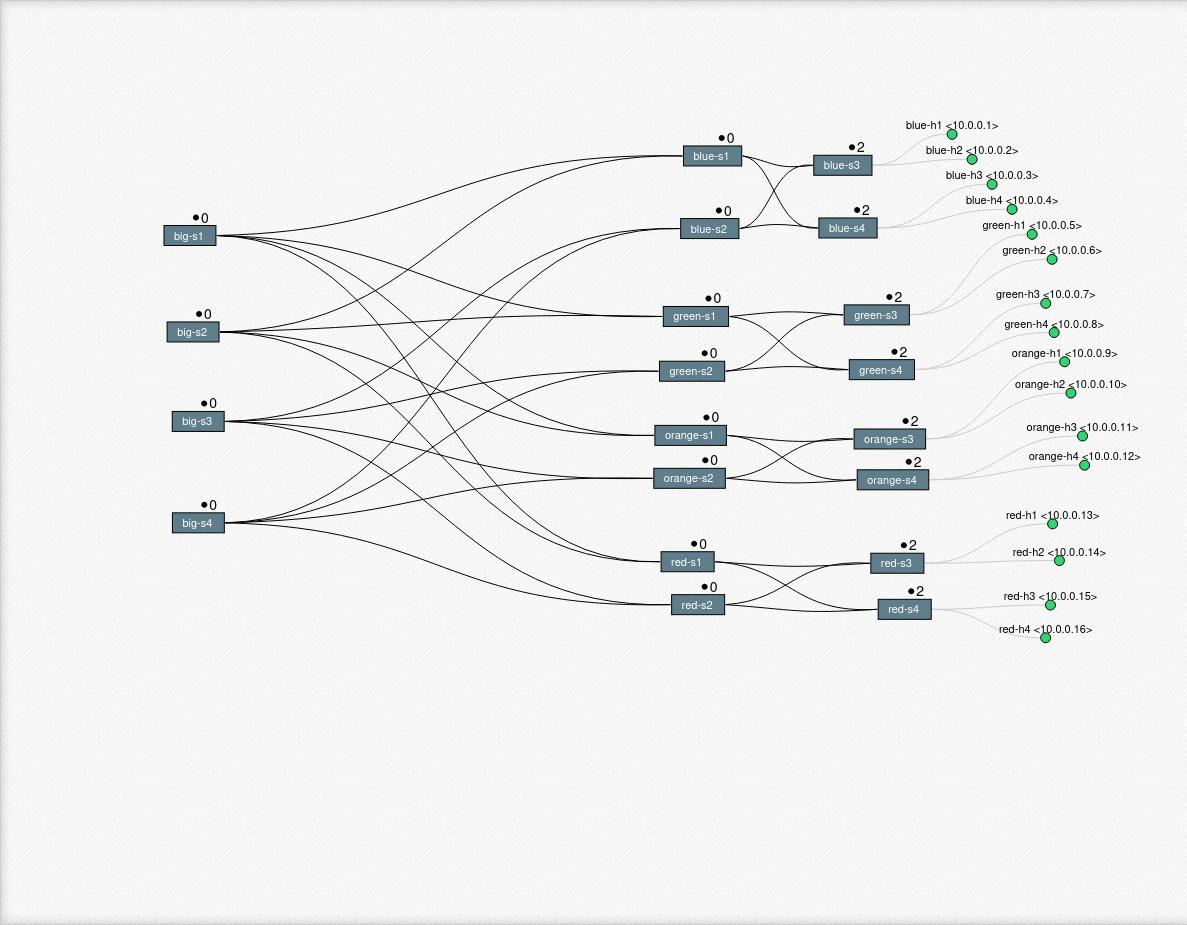
\includegraphics[width=1\linewidth]{images/exercise01-question02c.png}
            \caption{Fat Tree Topology on Mininet Topology Visualizer}
            \label{fig:placeholder}
        \end{figure}
    \end{center}

\end{document}Exercise 1